%!TEX root = ../main.tex
%%%%%%%%%%%%%%%%%%%%%%%%%%%%%%%%%%
% Links:
%
% Difficulty:
% Companies: 
%%%%%%%%%%%%%%%%%%%%%%%%%%%%%%%%%%


%\begin{figure}
%	\centering
%	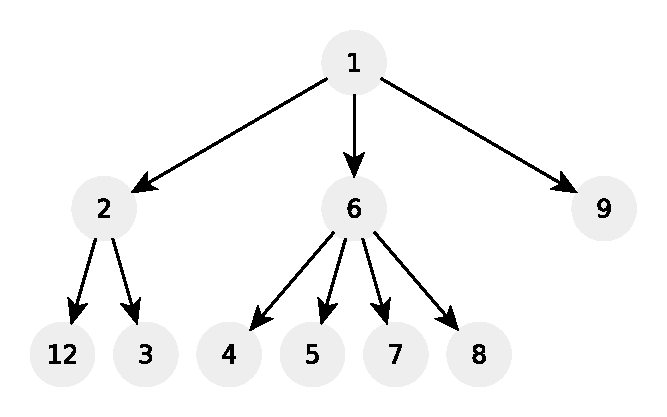
\includegraphics[width=\textwidth]{sources/gas_station/images/example1}
%	\caption[Sample short cpation]{Sample Caption}.
%	\label{fig:gas_station:example1}
%\end{figure}

\chapter{Gas Station \faGasPump}
\label{ch:gas_station}
\section*{Introduction}
Imagine there we drive along a circular route with a number of gas stations along it. Our goal is to drive across the entire route but before departure we would like to make sure we are not going to get stranded because we run out of gas.

Our car starts with an empty tank and can make 1km per 1l of gas and each gas station has a maximum amount of gas it can deliver. 
The problem with this setting is that we can end up in a situation where after 
having refueled we still do not have enough gas to reach the next gas station. 

In the problem discussed in this chapter we will discuss how to make sure  we always start the journey from a place along the route from where it is not possible to get stranded.


\section{Problem statement}
\begin{exercise}
\label{example:gas_station:exercice1}
You are given two arrays of integers $G$ and $C$ both of size $n$ 
where:
\begin{itemize}
	\item $G[i]$ represent the amount of gas station $i$ can deliver;
	\item and $C[i]$ is the amount of liters of gas necessary to reach the next gas station $i+1$;
\end{itemize}

You have a car with a tank of unlimited size and, you always start your journey from one of the gas stations and on an empty tank. 

You can only move forward from gas station $i$ to the next at index $i+1$. When you are at gas station $n-1$ you can travel to gas station $0$. 
A succesfull journey means starting at some gas station $k$, making $n$ stops for gas and ending up at gas station $k$.

Write a function that returns the smallest index $0 \leq k < n$ of a gas station from where you can start your journey and complete a loop around the circular route without getting stranded.

	%example1
	\begin{example}
		\label{example:gas_station:example1}
		\hfill \\
		Given $G=\{1,2\}$ and $C=\{2,1\}$ the function returns $1$(see Figure \ref{fig:gas_station:example1}).

		
        If we start from index $0$, we can fill in the tank with $G[0] = 1$ liters of gas. 
		Now our tank has $1$ liter of gas,	but we need $C[0] = 2$ gas to travel to station $1$. 
        
		If instead, we start from the station at index $1$, we can fill in $A[1] = 2$ liters of gas and end up with a tank with $2$ liters of gas. 
		We need only $B[1] = 1$ liters of gas to get to the next station $0$.
		We make the journey and travel to station $0$ and we still have $1$ unit of gas left. 
		At this point, we fill the tank again with $A[0] = 1$ liters of additional gas, for a total of $2$ liters in the tank. 
		It costs us $B[0] = 2$ liters to get to station $1$, which we do and we can then complete the loop succesfully. 
	\end{example}

	%example2
	\begin{example}
		\label{example:gas_station:example2}
		\hfill \\
		
		\hfill \\
		Given $G=\{7,1,0,11,4\}$ and $C=\{5,9,1,2,5\}$ the function returns $1$ (see Figure \ref{fig:gas_station:example2}).

		If we start our journey from the station $0$ we are stranded before we reach the station $2$. 
		If we start from station $1$ we cannot even make it to the next station as we can only fill the tank with $1$ liters but we need $9$ to reach station $2$. From staation $3$ it is clear we cannot make it because we cannot even refuel a drop of gas. 
		Station $3$ is the good one because we can fill the tank with $11$ liters, move to station $4$ only using $2$. At this point we can refuel $4$ liters and we set off with $13$ liters in the tank. Once we reach station $0$ we used $5$ but we can refill with $7$ and we are left with $15$.
		On the next leg we use $5$ liters of gas and refuel for $1$, leaving us with $11$ liters. On the next leg we use $11$ units but we do not get to refuel at all. At this point we are left with only $2$ liters of gas, but fortunately for the last leg of the trip we only need $1$ liter. 
		We therefore cirle back to the station $3$ with still $1$ liters left in the tank.

	\end{example}

\end{exercise}


\begin{figure}
	\centering
	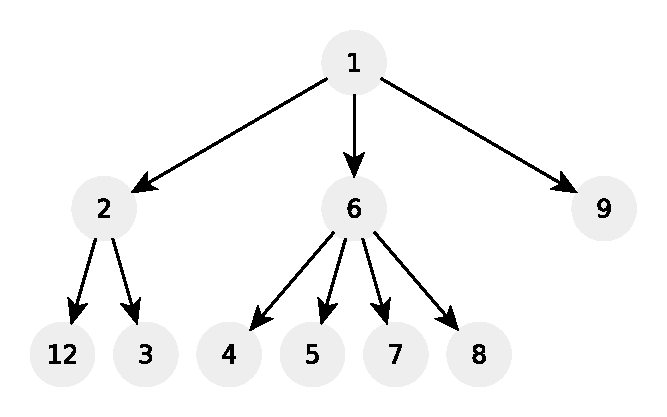
\includegraphics[width=\textwidth]{sources/gas_station/images/example1}
	\caption[Implicit graph for the Example \ref{example:gas_station:example1}.]
	{Visual representation the problem instance of Example
	\ref{example:gas_station:example1}.}.
	\label{fig:gas_station:example1}
\end{figure}

\begin{figure}
	\centering
	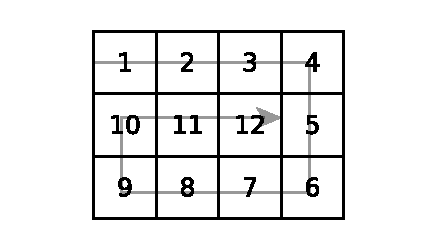
\includegraphics[width=\textwidth]{sources/gas_station/images/example2}
	\caption[Implicit graph for the Example \ref{example:gas_station:example2}.]
	{Visual representation the problem instance of Example
	\ref{example:gas_station:example2}.}.
	\label{fig:gas_station:example2}
\end{figure}

\section{Clarification Questions}

\begin{QandA}
	\item What shall the function return when it is not possible to complete a loop starting from any station? 
	\begin{answered}
		\textit{The function returns $-1$ in this case.}
	\end{answered}

	\item What is the maximum possible number of gas stations?
	\begin{answered}
		\textit{$n$ can be up to $1000000$.}
	\end{answered}

	\item Can we have negative values for gas refuel and cost?
	\begin{answered}
		\textit{No, you can assume $G$ and $C$ always contain non-negative integers.}
	\end{answered}
	
	\item Can $G$ and $C$ be empty?
	\begin{answered}
		\textit{Yes, $n$ can be zero.}
	\end{answered}
\end{QandA}

\section{Discussion}
\label{gas_station:sec:discussion}


\subsection{Brute-force}
\label{gas_station:sec:bruteforce}

\lstinputlisting[language=c++, caption={Brute-force solution.},label=list:gas_station]{sources/gas_station/gas_station_solution1.cpp}



\subsection{Linear time}
\label{gas_station:sec:linear_time}

\lstinputlisting[language=c++, caption={Brute-force solution.},label=list:gas_station]{sources/gas_station/gas_station_solution2.cpp}

